%---------------------------------------------------------------------
%
%                         Project Name:Njust LabReport 
%
%---------------------------------------------------------------------
%
%                 created by Qingyun Fang <fqy2017@gmail.com>
%
%                        Last-modified: 2017-6-12
%
%---------------------------------------------------------------------

\documentclass[a4paper,12pt]{report}
\usepackage{ctex}
%\usepackage{xeCJK}
\usepackage{times}
\usepackage{setspace}
\usepackage{fancyhdr}
\usepackage{graphicx}
\usepackage{wrapfig}
\usepackage{array}  
\usepackage{fontspec,xunicode,xltxtra}
\usepackage{titlesec}
\usepackage{titletoc}
\usepackage[titletoc]{appendix}
\usepackage[top=30mm,bottom=30mm,left=20mm,right=20mm]{geometry}
\usepackage{cite}
\usepackage{listings}
\usepackage[framed,numbered,autolinebreaks,useliterate]{mcode} % 插入代码
\XeTeXlinebreaklocale "zh"
\XeTeXlinebreakskip = 0pt plus 1pt minus 0.1pt

%---------------------------------------------------------------------
%	页眉页脚设置
%---------------------------------------------------------------------
\fancypagestyle{plain}{
	\pagestyle{fancy}      %改变章节首页页眉
}

\pagestyle{fancy}
\lhead{\kaishu~宜通华盛~}
\rhead{\kaishu~通信项目组~}
\cfoot{\thepage}

%---------------------------------------------------------------------
%	章节标题设置
%---------------------------------------------------------------------
\titleformat{\chapter}{\centering\zihao{-1}\heiti}{仿真实验\chinese{chapter}}{1em}{}
\titlespacing{\chapter}{0pt}{*0}{*6}

%---------------------------------------------------------------------
%	摘要标题设置
%---------------------------------------------------------------------
\renewcommand{\abstractname}{\zihao{-3} 摘\quad 要}

%---------------------------------------------------------------------
%	参考文献设置
%---------------------------------------------------------------------
\renewcommand{\bibname}{\zihao{2}{\hspace{\fill}参\hspace{0.5em}考\hspace{0.5em}文\hspace{0.5em}献\hspace{\fill}}}

%---------------------------------------------------------------------
%	引用文献设置为上标
%---------------------------------------------------------------------
\makeatletter
\def\@cite#1#2{\textsuperscript{[{#1\if@tempswa , #2\fi}]}}
\makeatother

%---------------------------------------------------------------------
%	目录页设置
%---------------------------------------------------------------------
\titlecontents{chapter}[0em]{\songti\zihao{-4}}{\thecontentslabel\ }{}
{\hspace{.5em}\titlerule*[4pt]{$\cdot$}\contentspage}
\titlecontents{section}[2em]{\vspace{0.1\baselineskip}\songti\zihao{-4}}{\thecontentslabel\ }{}
{\hspace{.5em}\titlerule*[4pt]{$\cdot$}\contentspage}
\titlecontents{subsection}[4em]{\vspace{0.1\baselineskip}\songti\zihao{-4}}{\thecontentslabel\ }{}
{\hspace{.5em}\titlerule*[4pt]{$\cdot$}\contentspage}


\begin{document}
%---------------------------------------------------------------------
%	封面设置
%---------------------------------------------------------------------
\begin{titlepage}
	\begin{center}
		
    
\includegraphics[width=0.9\textwidth]{figure//etws.png}\\
    \vspace{10mm}
    \textbf{\zihao{2}\kaishu{无线宽带自组网通信系统}}\\[0.8cm]
    \textbf{\zihao{2}\kaishu{ OLSR协议仿真实验报告}}\\[3cm]
    
	\vspace{\fill}
	
\setlength{\extrarowheight}{3mm}
{\songti\zihao{3}	
\begin{tabular}{rl}
	
	{\makebox[4\ccwd][s]{部\qquad 门:}}& ~\kaishu 研发部通信项目组\\
	
	{\makebox[4\ccwd][s]{姓\qquad 名:}}& ~\kaishu 罗敏 \\ 

\end{tabular}
 }\\[2cm]
\vspace{\fill}
\zihao{4}
使用\LaTeX 撰写于\today
	\end{center}	
\end{titlepage}

%---------------------------------------------------------------------
%  摘要页
%---------------------------------------------------------------------
\begin{abstract}
\begin{spacing}{1.5}
	{\zihao{-4}
	无人机集群是一个新的应用领域,特别是在军事领域,将会引发一场革命性的变革,而多机之间的通信又是无人机集群飞行之中的关键,如何实现
	更好的无几人集群之间的组网是一个需要深入研究和实验的方向。因应用领域的特殊性,真实环境采集数据测试具有很大的困难且花费大,因而需
	要预先实验仿真,本文档主要是仿真无人机集群使用olsr协议进行自组网通信,并评估olsr协议在组网过程中的各项性能指标和参数,为后续改进
	协议做参考。
	
	\textbf{关键字}:\quad 仿真 \quad 无人机集群 \quad olsr \quad 性能
	}
\end{spacing}
\end{abstract}

%---------------------------------------------------------------------
%  目录页
%---------------------------------------------------------------------
\tableofcontents % 生成目录

%---------------------------------------------------------------------
%  实验一
%---------------------------------------------------------------------
\chapter{路由生成与切换}
\setcounter{page}{1}
\begin{spacing}{1.5}
\songti\zihao{-4}

\section{实验目的}
本项实验主要目的有两个,具体如下:
\begin{itemize}
\itemsep=3pt
\parskip=0pt
\item 评估OLSR协议在整个无人机集群组网过程中路由生成时间
\item 评估OLSR协议拓扑变化时路由切换时间。
\end{itemize}
\section{实验工具}
本实验采用NS3仿真评估软件作为仿真工具,NS3平台提供了一套完成的协议仿真与数据记录工具,能够有效的仿真协议行为并在接近理想环境下评估协
议性能,需要了解更多详细信息可以参考NS3官方网站\cite{NS3.web}。
\section{实验设计}
根据实验目的,本实验采用如图1.1所示实验拓扑,每架无人机之间设置间隔距离500m,1号、2号和3号飞机相对静止,0号飞机进入飞行集群编队,
速度为20m/s,整个仿真过程60s,实时记录各个点之间通信报文并且每0.2秒打印一次每个节点的路由表变化情况,通过分析路由表变化记录可以得到
路由切换数据和路由生成数据。
\begin{figure}[hbtp]
	\centering
	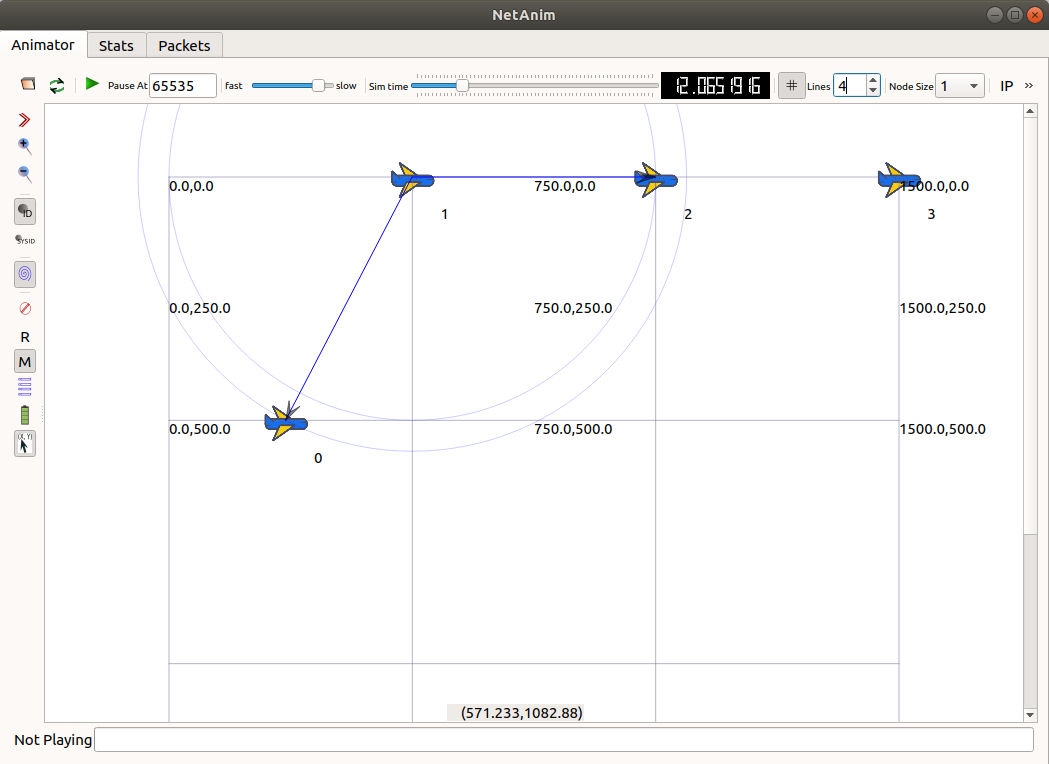
\includegraphics [width=0.8\textwidth]{figure//topo.png}
	\caption{仿真实验拓扑}\label{topo}
\end{figure}

\section{数据分析}
根据仿真采集的路由表数据分析后可得如图1.2和图1.3所示数据记录。
\section{实验结论}

\end{spacing}

%---------------------------------------------------------------------
%  实验二
%---------------------------------------------------------------------
\chapter{路由切换与数据传输}

\begin{spacing}{1.5}
\section{实验目的}

\section{实验工具}

\section{实验设计}

\section{实验内容}

\section{数据分析}

\section{实验结论}

\end{spacing}

%---------------------------------------------------------------------
%  实验感想
%---------------------------------------------------------------------
\titleformat{\chapter}{\centering\zihao{-1}\heiti}{}{1em}{}
\chapter{实验总结}
\begin{spacing}{1.5}
	没什么好说的。
\end{spacing}

%---------------------------------------------------------------------
%  参考文献设置
%---------------------------------------------------------------------
\addcontentsline{toc}{chapter}{参考文献}

\begin{thebibliography}{99}
\songti \zihao{-4} 	
	\bibitem{Leslie.{1994}}
	Leslie Lamport. LATEX: A Document Preparation System.AddisonWesley, Reading, Massachusetts, second edition, 1994, ISBN 0-201-52983-1.
	
	\bibitem{Donald.{1984}}
	Donald E. Knuth. The TEXbook, Volume A of Computers and Typesetting,Addison Wesley, Reading, Massachusetts, second edition, 1984,ISBN 0-201-13448-9.

	\bibitem{NS3.web}
	https://www.nsnam.org/
	
\end{thebibliography}

%---------------------------------------------------------------------
%  附录设置
%---------------------------------------------------------------------
\titleformat{\chapter}{\heiti\Large}{附录~\Alph{chapter}}{11pt}{\Large}
\titlespacing{\chapter}{0pt}{*-4}{*4}

\lstset{breaklines}                %自动将长的代码行换行排版
\lstset{extendedchars=false}
\lstset{language=Matlab}
\renewcommand{\thechapter}{附录\Alph{chapter}.} 
\appendix
\begin{appendix}
	
	
\chapter{数据表}
\zihao{-4}\songti
\begin{spacing}{1.5}
	hello world!
\end{spacing}


\chapter{程序代码}
\zihao{-4}\songti
\begin{spacing}{1.5}
下面是一个MATLAB程序的事例,使用了Package mcode,它能较好还原MATLAB本身的编写风格。
\begin{lstlisting}
%The program normalizes the measurement data and compares it to the standard cosine function
data=xlsread('data_sun',1,'B3:E39');
min=[(data(1,1)+data(37,1))/2,(data(1,2)+data(37,2))/2,...
(data(1,3)+data(37,3))/2,(data(1,4)+data(37,4))/2];
max=[data(19,1),data(19,2),data(19,3),data(19,4)];
Min=repmat(min,37,1);
Max=repmat(max,37,1);
data=(data-Min)./(Max-Min);
x=-pi/2:pi/36:pi/2;
y=cos(x);
%----------------------figure-------------------------%
figure(1);
subplot(2,2,1);
plot(x,data(:,1),'ro-');
hold on;
plot(x,y,'b-');
title('R=1.2\Omega');
axis([-2,2,0,1]);
grid on;
subplot(2,2,2);
plot(x,data(:,2),'ro-');
hold on;
plot(x,y,'b-');
title('R=1.6\Omega');
axis([-2,2,0,1]);
grid on;
subplot(2,2,3);
plot(x,data(:,2),'ro-');
hold on;
plot(x,y,'b-');
title('R=2.0\Omega');
axis([-2,2,0,1]);
grid on;
subplot(2,2,4);
plot(x,data(:,4),'ro-');
hold on;
plot(x,y,'b-');
title('R=2.4\Omega');
grid on;
axis([-2,2,0,1]);
\end{lstlisting}
\end{spacing}
\end{appendix}
		

\end{document}